The Linear Kernel SVM had the worst performance in comparison to the others.
This fact can be seen in Table \ref{tab:linear_SVM}, in which is observed that
this machine does not classify any data point to the class 1 as the sensitivity
value is 0 for the three datasets.

\begin{table}
  \centering
  \caption{Performance scores for linear SVM.}
  \label{tab:linear_SVM}
  \begin{tabular}{ccc}
    \hline
    \textbf{Set} & \textbf{Sensitivity} & \textbf{Specificity} \\ \hline
    Training & 0 & 1 \\
    Testing & 0 & 1 \\
    Validation & 0 & 1 \\ \hline
  \end{tabular}
\end{table}

The fact that the Linear Kernel SVM could not learn the training data set shows
us, intuitively, that the data set is not linearly separable and that the data
set has some non-linearities that heavily difficult the learning of it.
Furthermore, in Fig. \ref{fig:SVM-linear} it is seen that in each of the
projections the decision function for the linear kernel SVM is always negative.

\begin{figure*}
  \centering
  \begin{subfigure}[b]{0.32\textwidth}
    \centering
    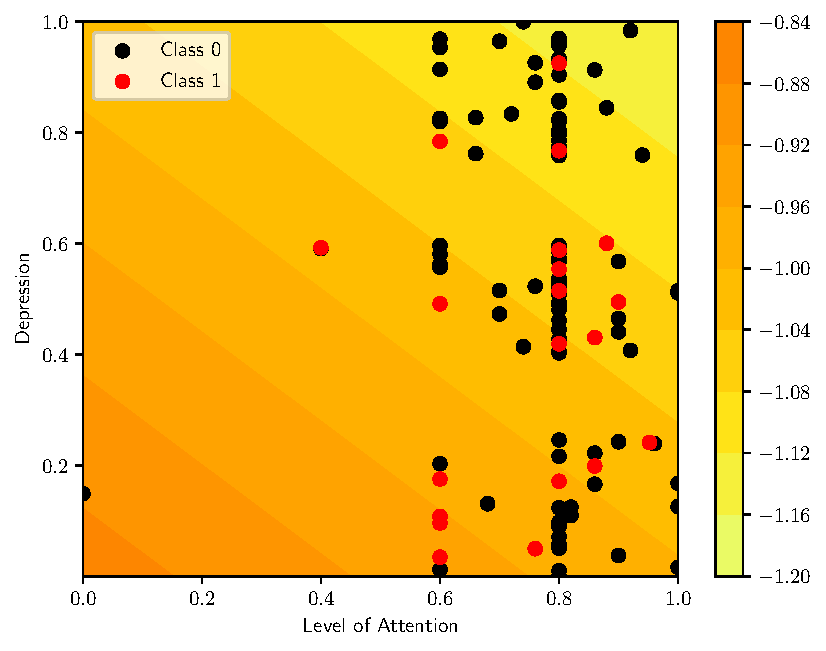
\includegraphics[width=\textwidth]{figs/svm-linear-contour-0-3.pdf}
    \caption{}
    \label{fig:SVM-linear1a}
  \end{subfigure}
  \begin{subfigure}[b]{0.32\textwidth}
    \centering
    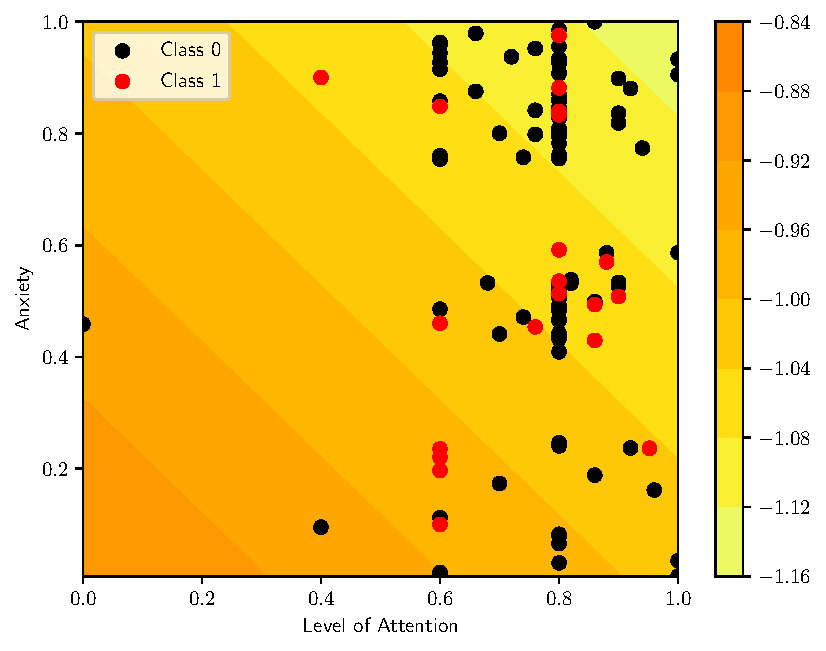
\includegraphics[width=\textwidth]{figs/svm-linear-contour-0-4.pdf}
    \caption{}
  \end{subfigure}
  \begin{subfigure}[b]{0.32\textwidth}
    \centering
    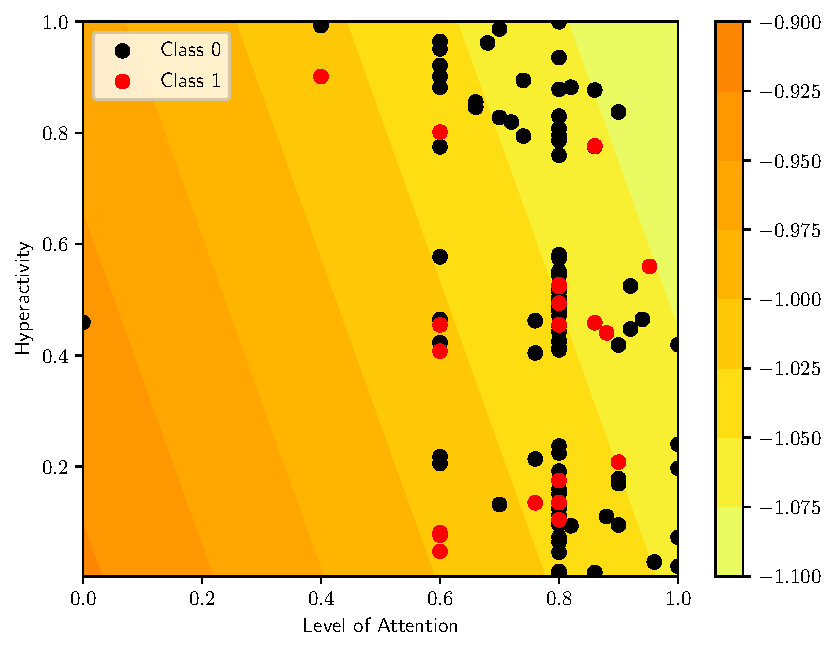
\includegraphics[width=\textwidth]{figs/svm-linear-contour-0-5.pdf}
    \caption{}
    \label{fig:SVM-linear1c}
  \end{subfigure}

  \begin{subfigure}[b]{0.32\textwidth}
    \centering
    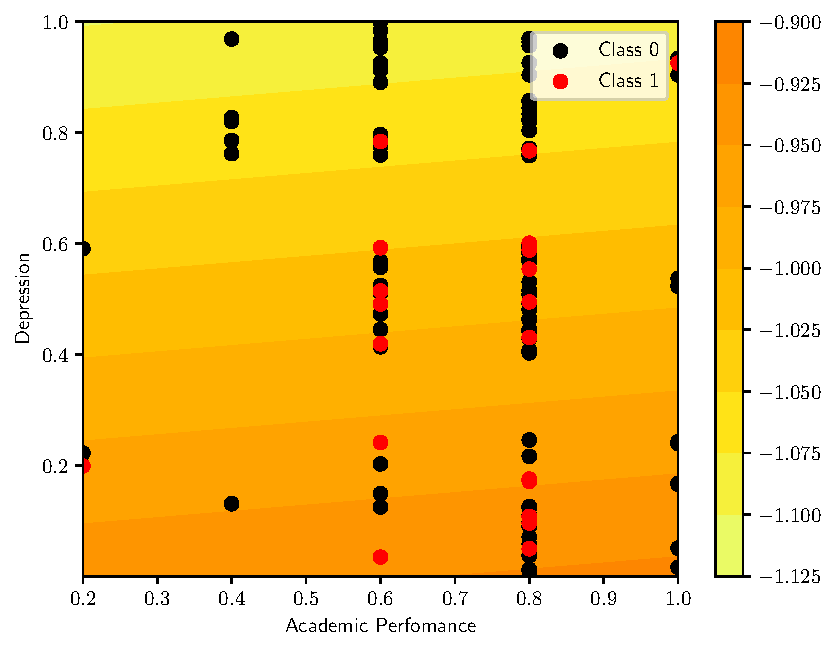
\includegraphics[width=\textwidth]{figs/svm-linear-contour-1-3.pdf}
    \caption{}
    \label{fig:SVM-linear2a}
  \end{subfigure}
  \begin{subfigure}[b]{0.32\textwidth}
    \centering
    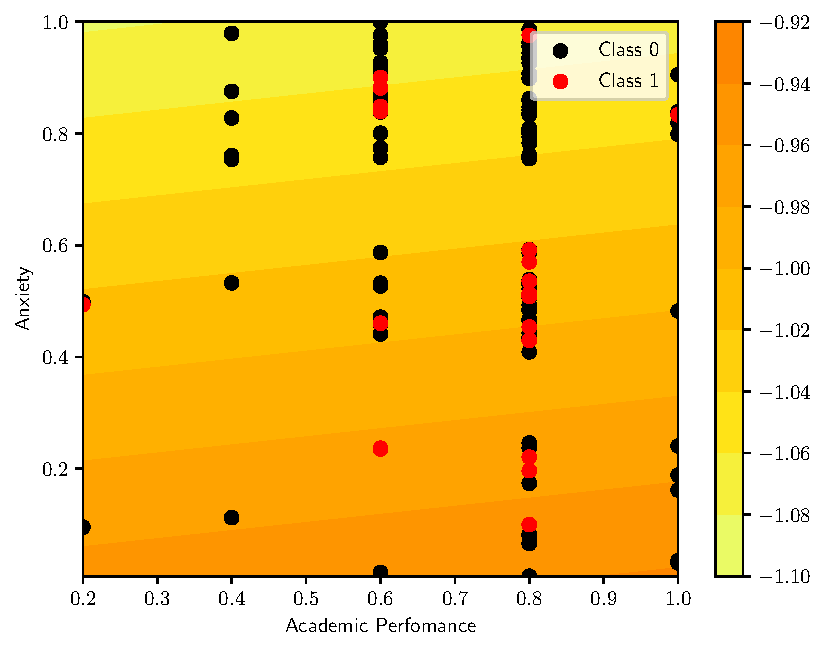
\includegraphics[width=\textwidth]{figs/svm-linear-contour-1-4.pdf}
    \caption{}
  \end{subfigure}
  \begin{subfigure}[b]{0.32\textwidth}
    \centering
    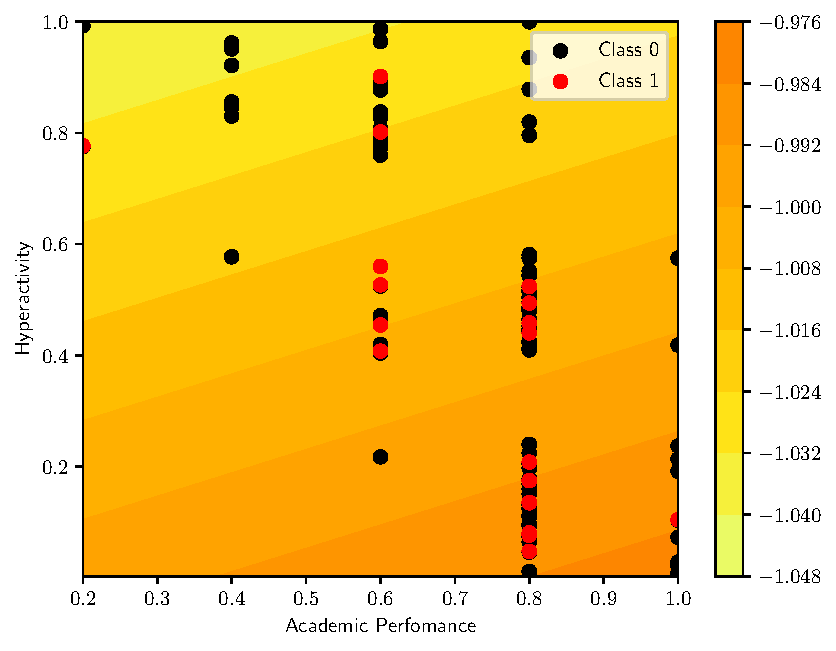
\includegraphics[width=\textwidth]{figs/svm-linear-contour-1-5.pdf}
    \caption{}
    \label{fig:SVM-linear2c}
  \end{subfigure}

  \begin{subfigure}[b]{0.32\textwidth}
    \centering
    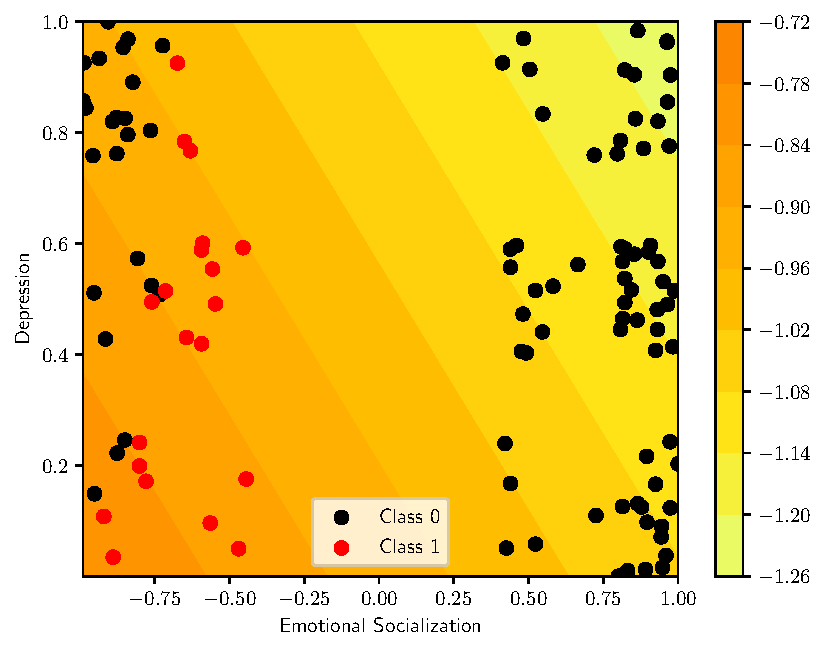
\includegraphics[width=\textwidth]{figs/svm-linear-contour-2-3.pdf}
    \caption{}
  \end{subfigure}
  \begin{subfigure}[b]{0.32\textwidth}
    \centering
    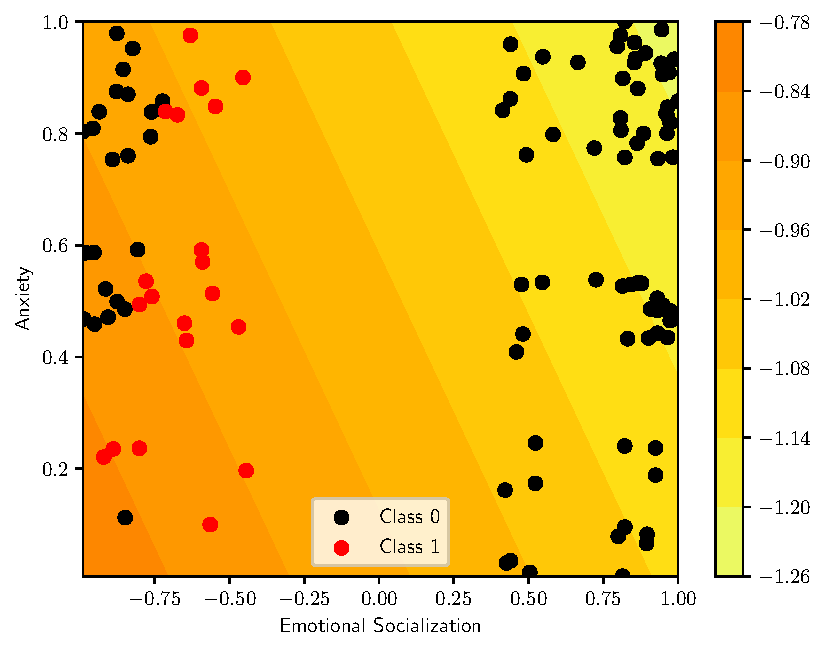
\includegraphics[width=\textwidth]{figs/svm-linear-contour-2-4.pdf}
    \caption{}
  \end{subfigure}
  \begin{subfigure}[b]{0.32\textwidth}
    \centering
    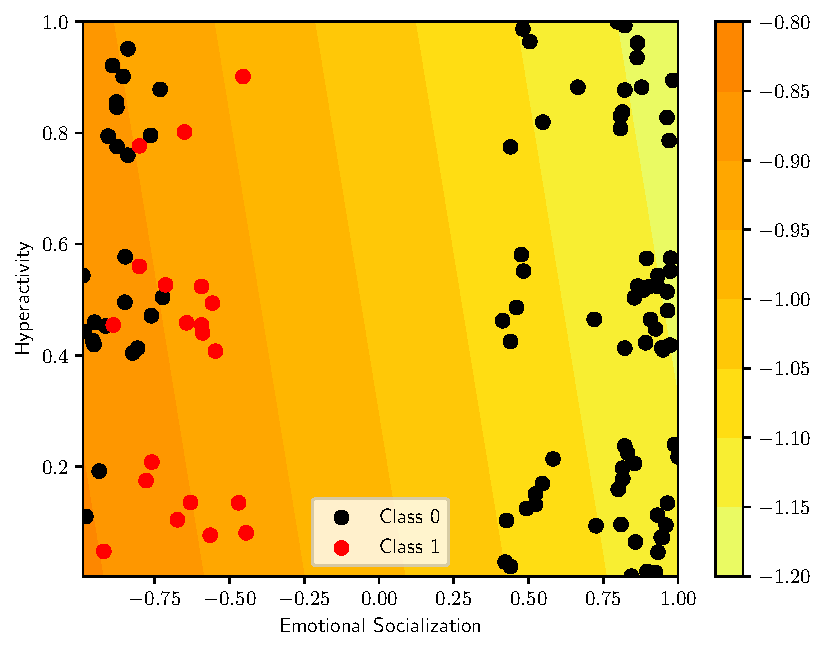
\includegraphics[width=\textwidth]{figs/svm-linear-contour-2-5.pdf}
    \caption{}
  \end{subfigure}
  \caption{Linear kernel SVM contour with real labels.}
  \label{fig:SVM-linear}
\end{figure*}

On the other hand, it is important to remark the contours still preserve a
linear structure. This fact assures us that the procedure for which these
contours are calculated can, partially, represent what's happening in higher
dimensions.

Lastly, it is also seen that in Figs.
\ref{fig:SVM-linear1a}-\ref{fig:SVM-linear1c},
\ref{fig:SVM-linear2a}-\ref{fig:SVM-linear2c} that the data are sparsed over
some discrete lines. This also verifies the realized projection as the variables
of this figures are discrete.

\begin{figure*}
    \centering
    \begin{subfigure}[b]{0.32\textwidth}
        \centering
        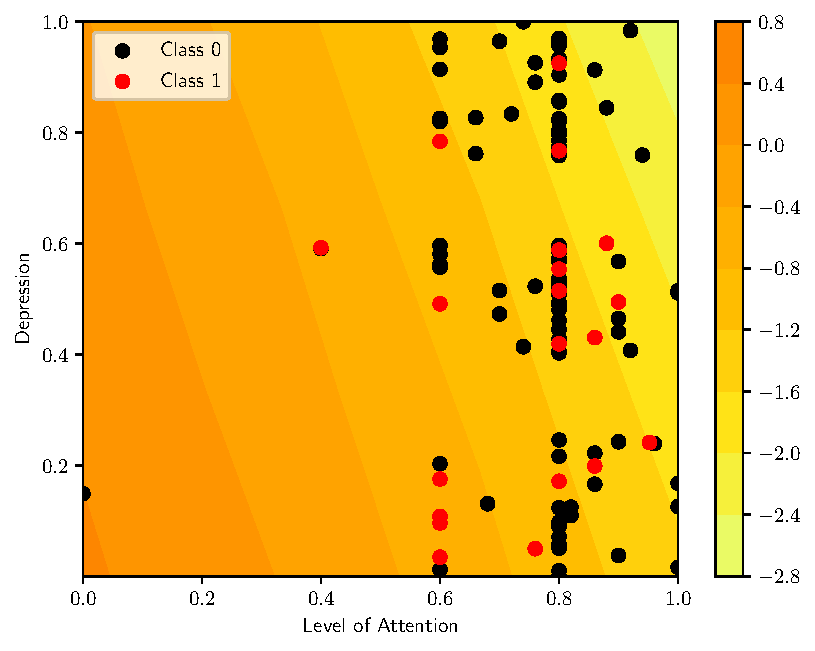
\includegraphics[width=\textwidth]{figs/svm-poly-contour-0-3.pdf}
        \caption{}
    \end{subfigure}
    \begin{subfigure}[b]{0.32\textwidth}
        \centering
        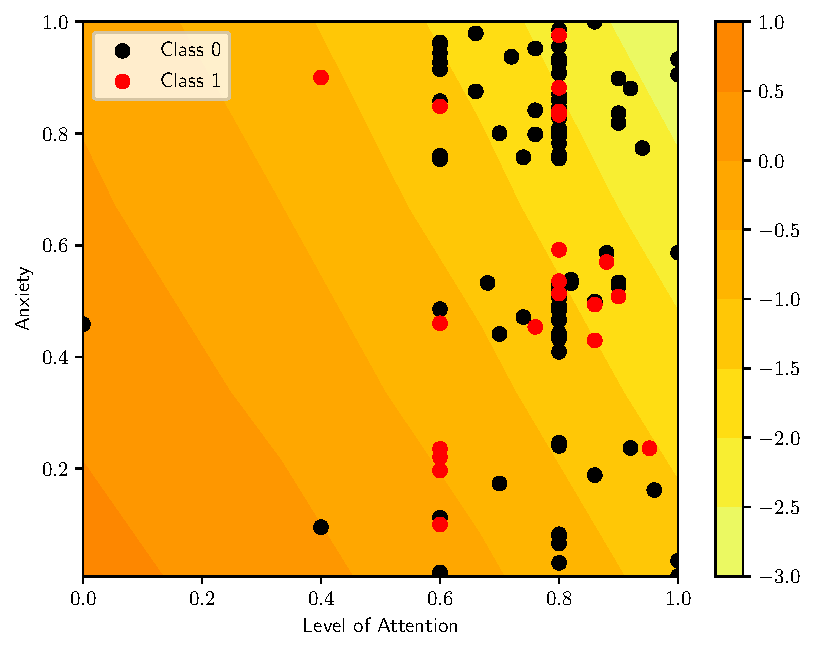
\includegraphics[width=\textwidth]{figs/svm-poly-contour-0-4.pdf}
        \caption{}
    \end{subfigure}
    \begin{subfigure}[b]{0.32\textwidth}
        \centering
        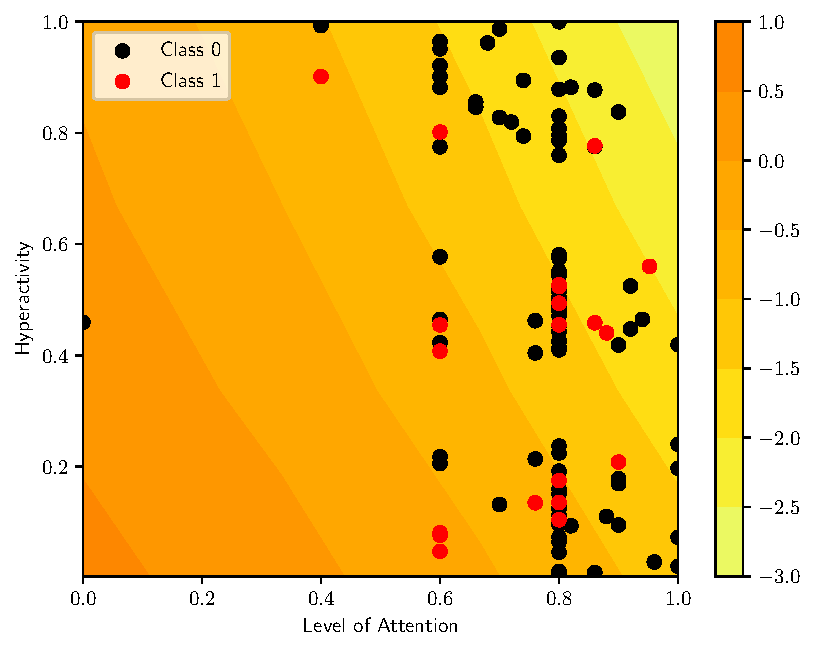
\includegraphics[width=\textwidth]{figs/svm-poly-contour-0-5.pdf}
        \caption{}
    \end{subfigure}

    \begin{subfigure}[b]{0.32\textwidth}
        \centering
        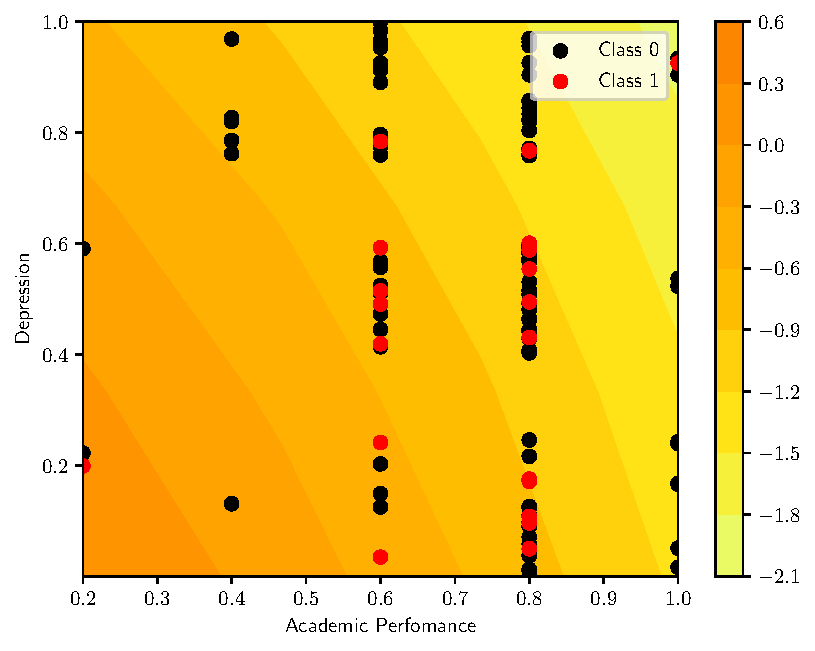
\includegraphics[width=\textwidth]{figs/svm-poly-contour-1-3.pdf}
        \caption{}
    \end{subfigure}
    \begin{subfigure}[b]{0.32\textwidth}
        \centering
        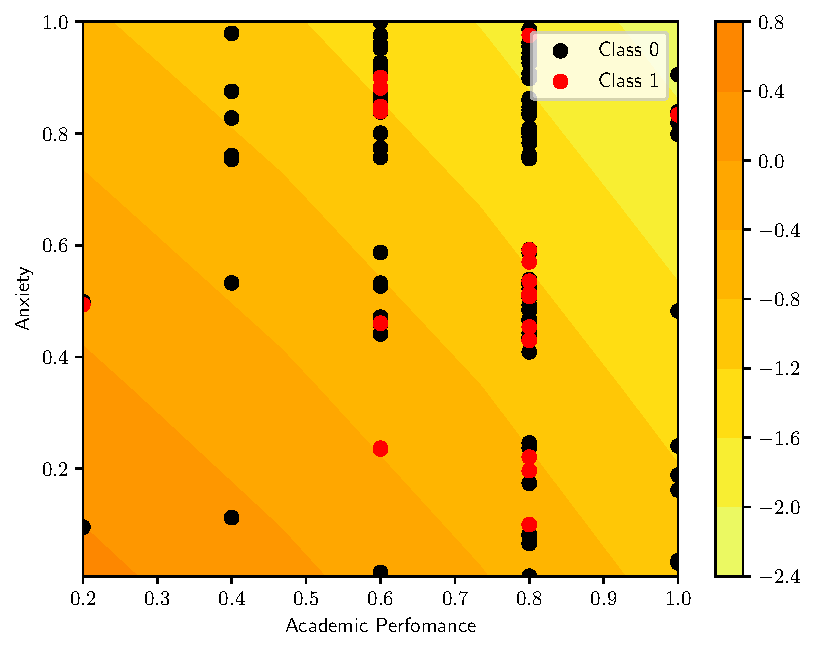
\includegraphics[width=\textwidth]{figs/svm-poly-contour-1-4.pdf}
        \caption{}
    \end{subfigure}
    \begin{subfigure}[b]{0.32\textwidth}
        \centering
        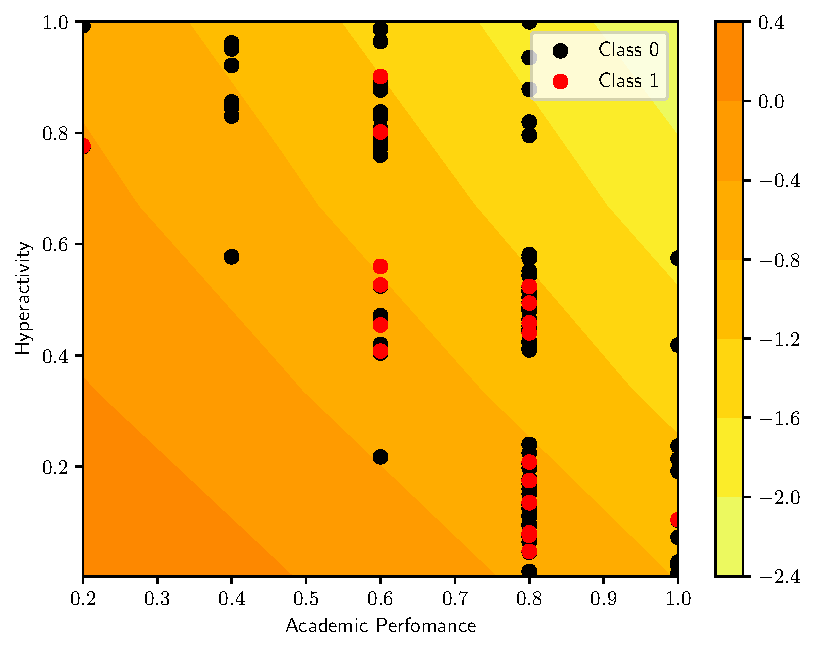
\includegraphics[width=\textwidth]{figs/svm-poly-contour-1-5.pdf}
        \caption{}
    \end{subfigure}

    \begin{subfigure}[b]{0.32\textwidth}
        \centering
        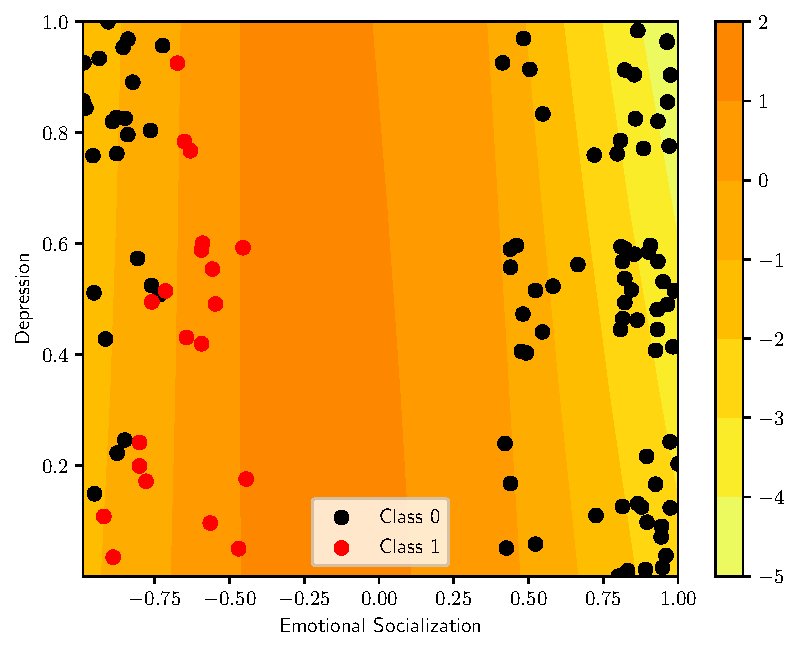
\includegraphics[width=\textwidth]{figs/svm-poly-contour-2-3.pdf}
        \caption{}
    \end{subfigure}
    \begin{subfigure}[b]{0.32\textwidth}
        \centering
        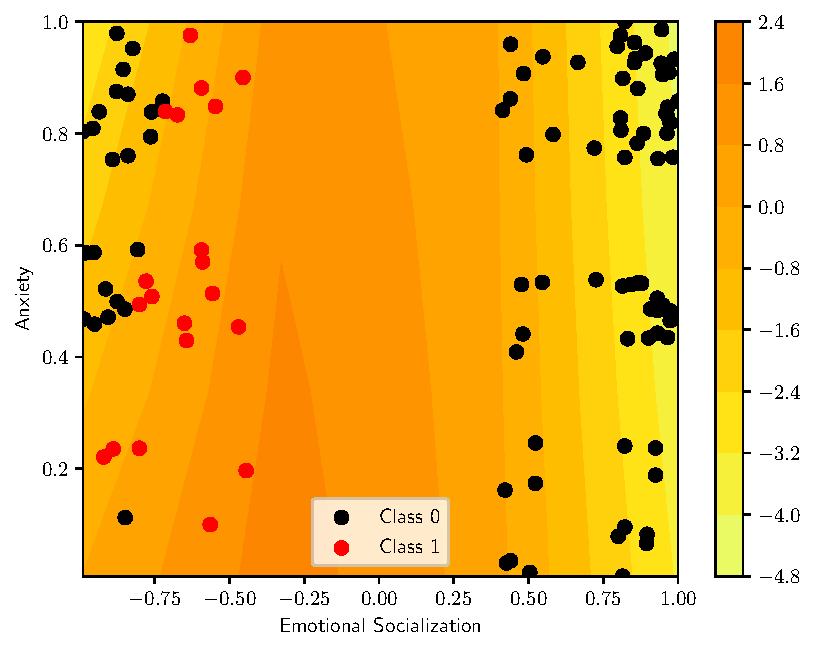
\includegraphics[width=\textwidth]{figs/svm-poly-contour-2-4.pdf}
        \caption{}
    \end{subfigure}
    \begin{subfigure}[b]{0.32\textwidth}
        \centering
        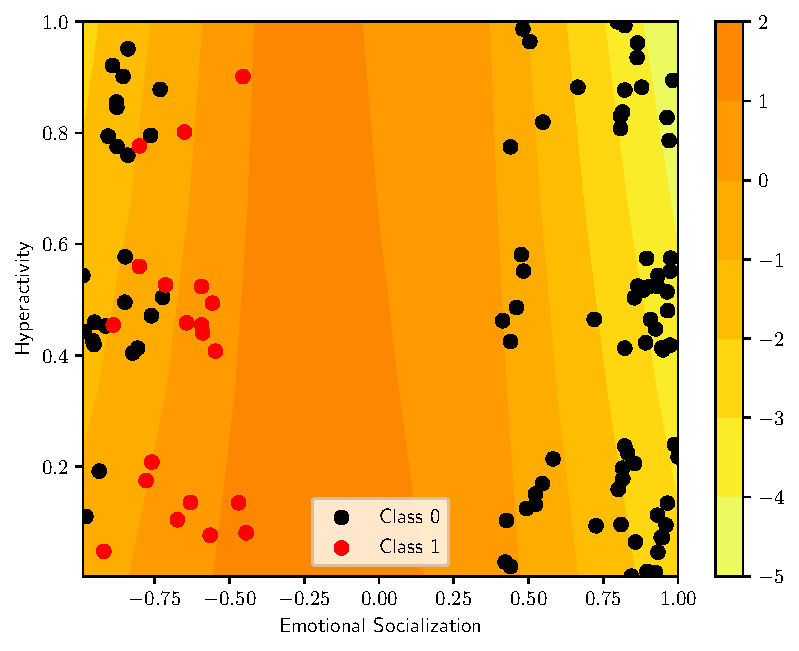
\includegraphics[width=\textwidth]{figs/svm-poly-contour-2-5.pdf}
        \caption{}
    \end{subfigure}
    \caption{Polynomial kernel SVM contour with real labels.}
    \label{fig:SVM-poly}
\end{figure*}

\begin{figure*}
    \centering
    \begin{subfigure}[b]{0.32\textwidth}
        \centering
        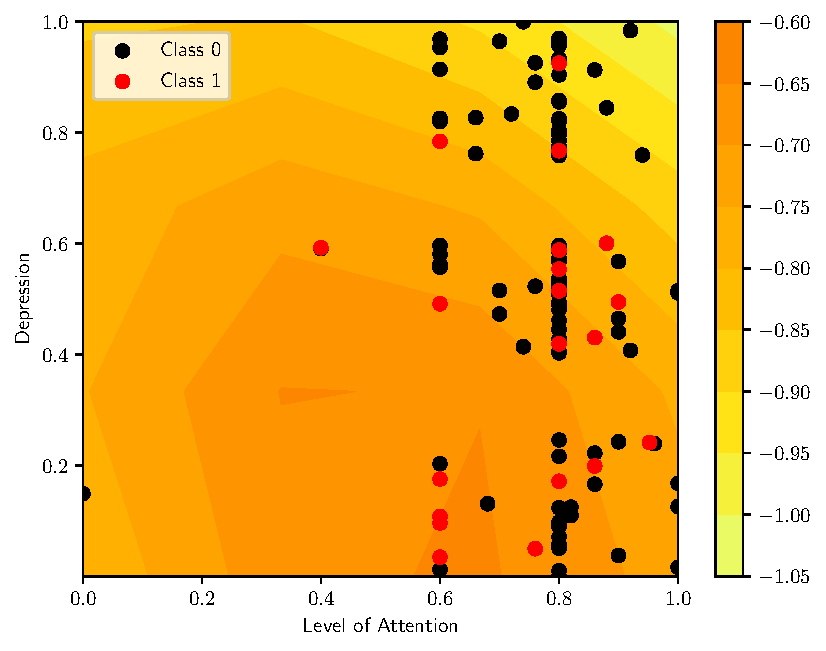
\includegraphics[width=\textwidth]{figs/svm-rbf-contour-0-3.pdf}
        \caption{}
    \end{subfigure}
    \begin{subfigure}[b]{0.32\textwidth}
        \centering
        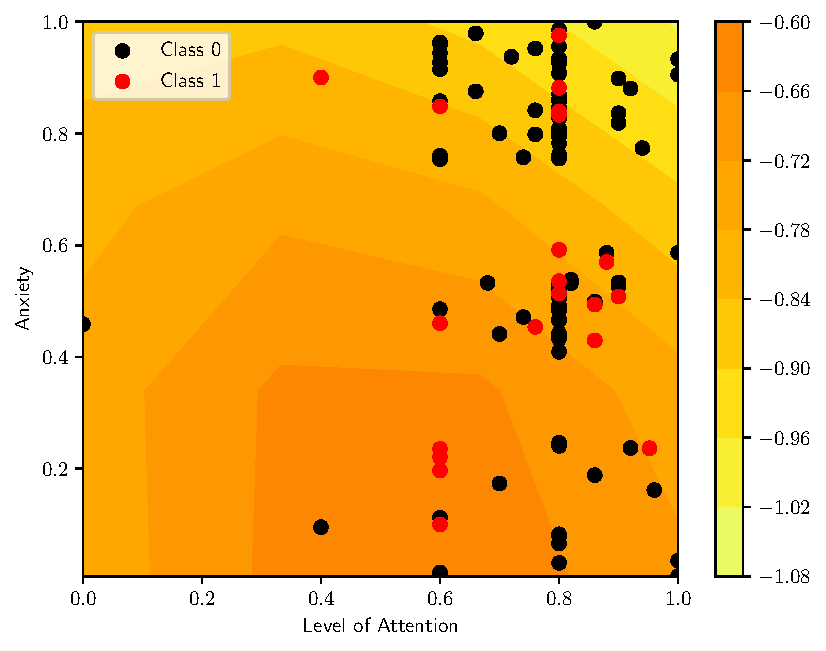
\includegraphics[width=\textwidth]{figs/svm-rbf-contour-0-4.pdf}
        \caption{}
    \end{subfigure}
    \begin{subfigure}[b]{0.32\textwidth}
        \centering
        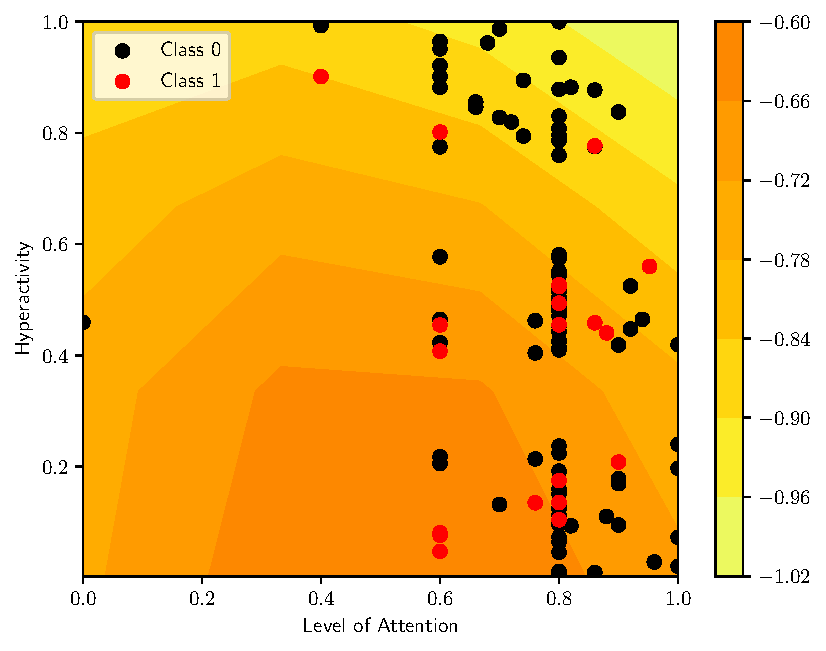
\includegraphics[width=\textwidth]{figs/svm-rbf-contour-0-5.pdf}
        \caption{}
    \end{subfigure}

    \begin{subfigure}[b]{0.32\textwidth}
        \centering
        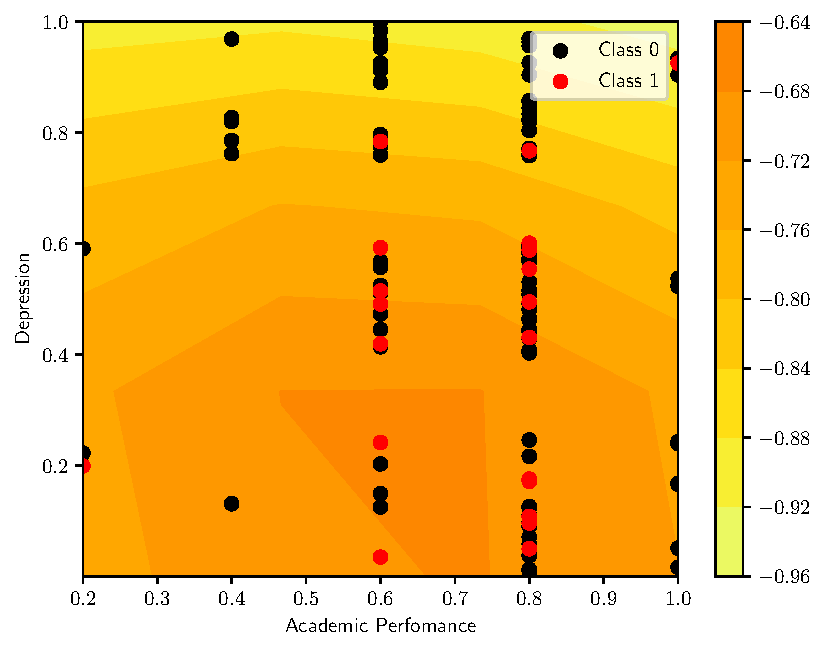
\includegraphics[width=\textwidth]{figs/svm-rbf-contour-1-3.pdf}
        \caption{}
    \end{subfigure}
    \begin{subfigure}[b]{0.32\textwidth}
        \centering
        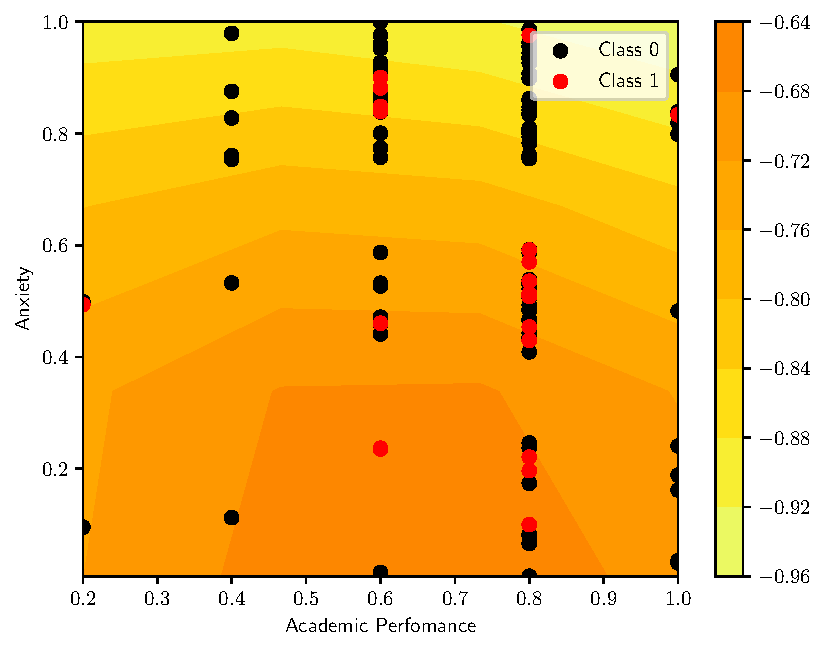
\includegraphics[width=\textwidth]{figs/svm-rbf-contour-1-4.pdf}
        \caption{}
    \end{subfigure}
    \begin{subfigure}[b]{0.32\textwidth}
        \centering
        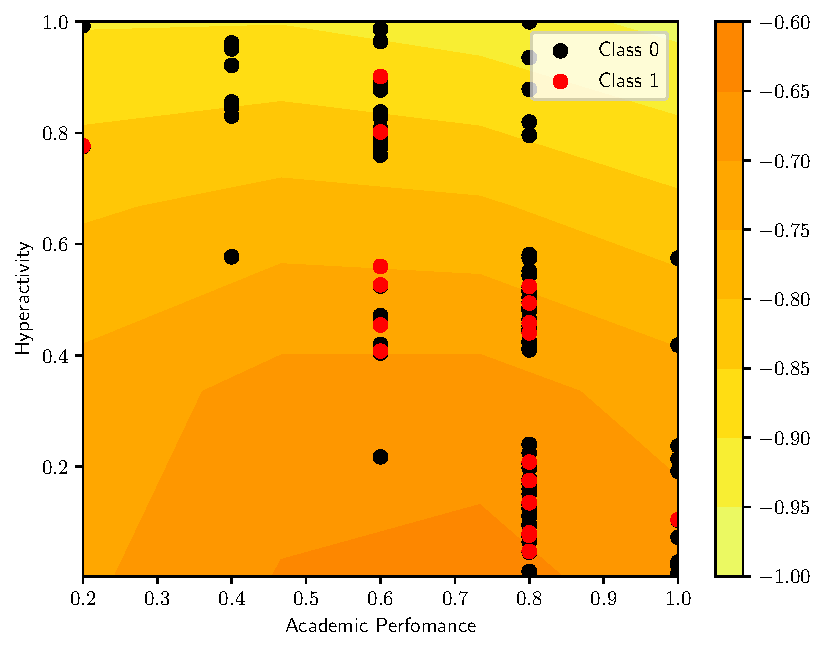
\includegraphics[width=\textwidth]{figs/svm-rbf-contour-1-5.pdf}
        \caption{}
    \end{subfigure}

    \begin{subfigure}[b]{0.32\textwidth}
        \centering
        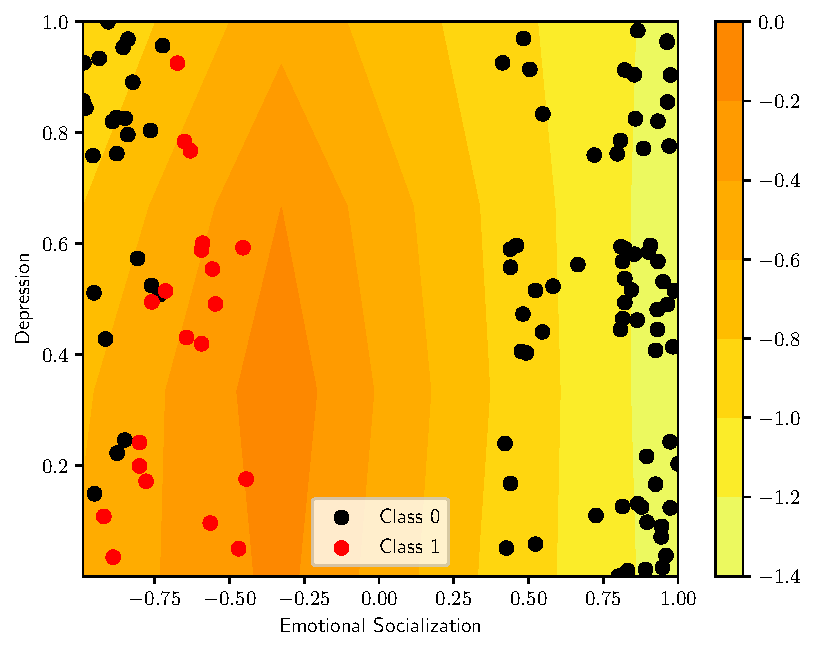
\includegraphics[width=\textwidth]{figs/svm-rbf-contour-2-3.pdf}
        \caption{}
    \end{subfigure}
    \begin{subfigure}[b]{0.32\textwidth}
        \centering
        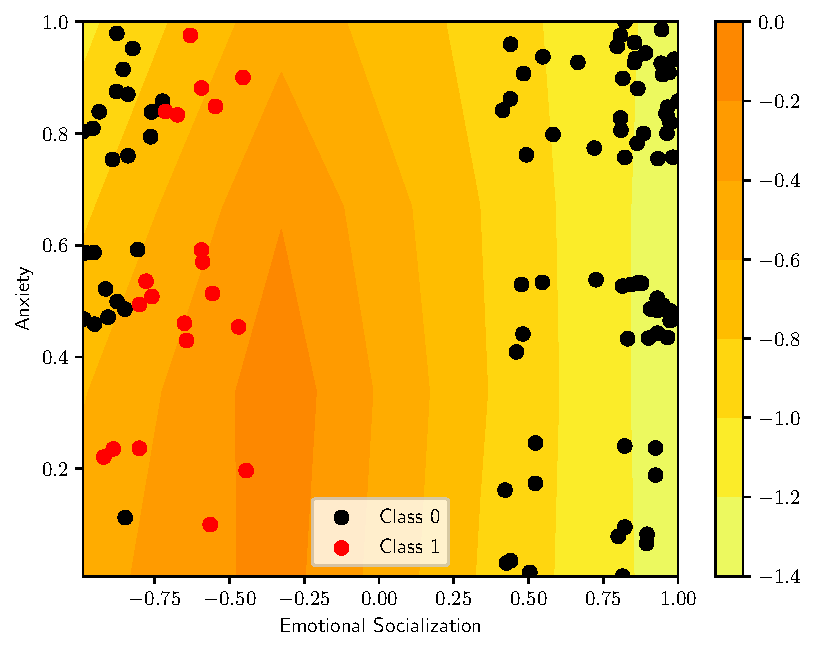
\includegraphics[width=\textwidth]{figs/svm-rbf-contour-2-4.pdf}
        \caption{}
    \end{subfigure}
    \begin{subfigure}[b]{0.32\textwidth}
        \centering
        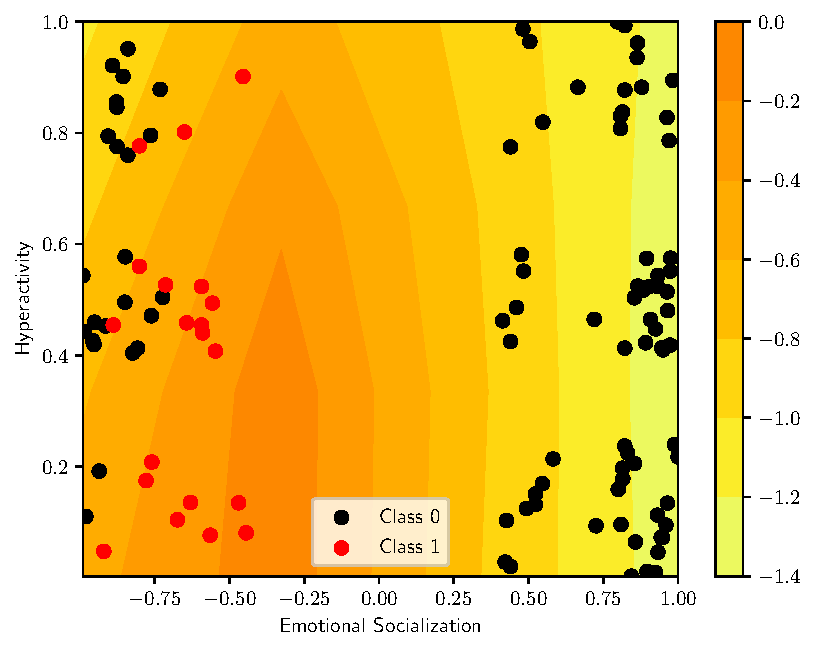
\includegraphics[width=\textwidth]{figs/svm-rbf-contour-2-5.pdf}
        \caption{}
    \end{subfigure}
    \caption{RBF kernel SVM contour with real labels.}
    \label{fig:SVM-rbf}
\end{figure*}

\begin{table}
\centering
\caption{Performance scores for polynomial SVM.}
\label{tab:poly_SVM}
\begin{tabular}{cll}
\hline
\textbf{Set} & \multicolumn{1}{c}{\textbf{Sensitivity}} & \multicolumn{1}{c}{\textbf{Specificity}} \\ \hline
Training & 0.89 & 1 \\
Testing & 0 & 1 \\
Validation & 0.57 & 1 \\ \hline
\end{tabular}
\end{table}

\begin{table}
\centering
\caption{Performance scores for RBF SVM.}
\label{tab:rbf_SVM}
\begin{tabular}{cll}
\hline
\textbf{Set} & \multicolumn{1}{c}{\textbf{Sensitivity}} & \multicolumn{1}{c}{\textbf{Specificity}} \\ \hline
Training & 0.13 & 1 \\
Testing & 0 & 1 \\
Validation & 0.25 & 1 \\ \hline
\end{tabular}
\end{table}
